\documentclass{report}
\usepackage{graphicx}
\usepackage[export]{adjustbox}

\title{Stonks \large \\
A game about making money from buying and selling stocks}
\author{Ezequiel Torres}


\begin{document}
\maketitle 
\begin{itemize}
    \item Game Design Document Template
    \item Version v1.0, June 14 2024\\
\end{itemize}
\newpage

\begin{abstract}
You will compete against bots in an all out brawl of purchasing and selling stocks. You will start with a small loan of 500 dollars, which is an average price of a stock. You will need to analyze the stock graphs to see when is a good time to purchase a stock, then you will need to make a sell for profit. Your end goal is to have more capital than your opponents and to bankrupt them.
\end{abstract}

\tableofcontents

% ______________________
% chapter Overview
% ______________________
\chapter{Overview}

The main features of the game are as follows. Purchasing and selling stocks, which need to contribute to the stock value. Each stock will need to be its own object which is tracked in a graph that the user can view. 

The game will also feature bots, which will be able to purchase and sell stocks based on their capital. This of course will also contribute to the value of the stocks. 

We will need a game loop. This game loop will include viewing seperate stock graphs, ending the day, and purchasing and selling stocks. The end goal is to bankrupt your opponents and the way to accomplish this is to out bid them until they run out of capital. 

\section{Main Concept}
The main concept is.. (WIP).

\section{Graphics}
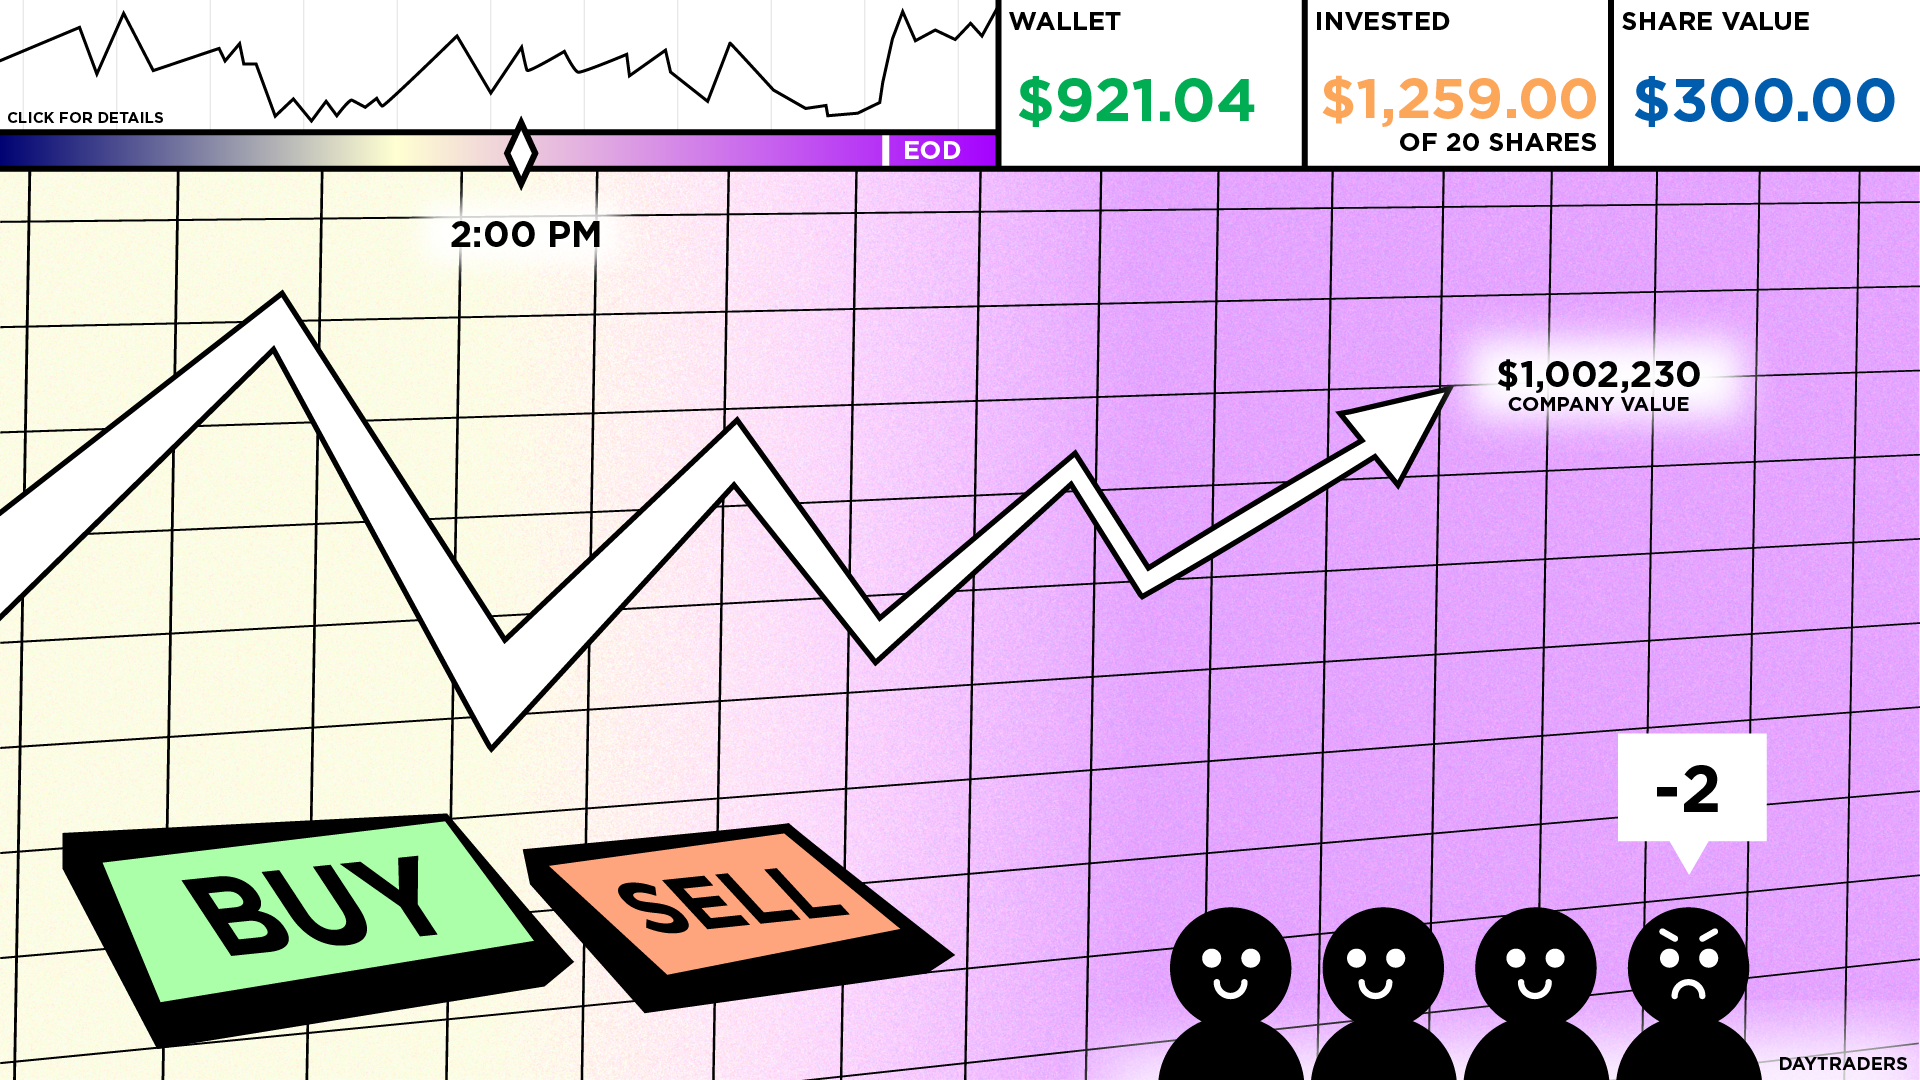
\includegraphics[max size={\textwidth}{\textheight}]{Devin-Base-Graphic.png}


\end{document}
